\subsection{Model summary}

Understanding of the database and the structure of the Company is essential to understanding the code.

As described in Clause 1 (page 10): 

\begin{quotation}
    The Company portrayed by the benchmark is a wholesale supplier with a number of geographically distributed sales districts and associated warehouses. As the Company's business expands, new warehouses and associated sales districts are created. Each regional warehouse covers 10 districts. Each district serves 3,000 customers. All warehouses maintain stocks for the 100,000 items sold by the Company. The following diagram illustrates the warehouse, district, and customer hierarchy of TPC-C's business environment. 
    
\end{quotation}

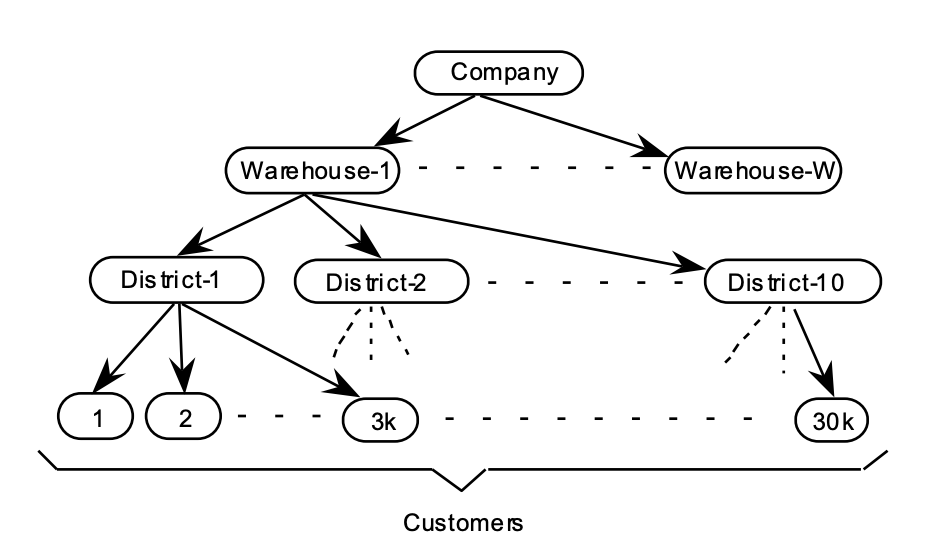
\includegraphics{img/model.png}
    
\begin{quotation}
    Customers call the Company to place a new order or request the status of an existing order. Orders are composed of an average of 10 order lines (i.e. line items). One percent of all order lines are for items not in-stock at the regional warehouse and must be supplied by another warehouse. 

    The Company's system is also used to enter payments from customers, process orders for delivery, and examine stock levels to identify potential supply shortages.
\end{quotation}

\subsection{Abridged table chema}
\textit{The TPC-C database contains nine tables. Primary keys are bolded and underlined below.}

WAREHOUSE(\underline{\textbf{wId}}, name, str1, str2, city, state, zip, tax, wYTD)

DISTRICT(\underline{\textbf{dId, wId*}}, name, str1, str2, city, state, zip, tax,  dYTD, nextOrdId)

CUSTOMER(\underline{\textbf{cId, dId, wId}}, first, middle, last, str1, str2, city, state, zip, phone, since, credit, creditLim, discount, balance, YTDPaymt, paymtCnt, deliveryCnt, data)

HISTORY(cId, cDId, cWId, dId, wId, date, amount, data)

NEWORDER(\underline{\textbf{oId, dId, wId}})

ORDER(\underline{\textbf{oId, dId*, wId*}}, cId*, entryDate, carrierId, oLCnt, allLocal)

ORDERLINE(\underline{\textbf{oId, dId*, wId*, number}}, iId, supplyWId, deliveryDate, quantity, amount, distInfo)

ITEM(\underline{\textbf{iId}}, iMId, name, price, data)

STOCK(\underline{\textbf{iId*, wId*}}, quantity, dist01, dist02, dist03, dist04, dist05, dist06, dist07, dist08, dist09, dist10, YTD, orderCnt, remoteCnt, data)



\textbf{Foreign keys:}

DISTRICT(wId) references  WAREHOUSE(wId)

CUSTOMER(wId, dId) references DISTRICT(wId, dId)

HISTORY(cWId, cDId, cId) references CUSTOMER(wId, dId, cId)

HISTORY (wId, dId) references DISTRICT(wId, dId) 

NEWORDER(wId, dId, oId) references ORDER(wId, dId, oId)

ORDER (wId, dId, cId)  references CUSTOMER(wId, dId, cId)

ORDERLINE(wId, dId, oId) references ORDER(wId, dId, oId)

ORDERLINE(supplyWId, iId) references STOCK(wId, iId)

STOCK(wId) references WAREHOUSE(wId) 

STOCK(iId) references ITEM(iId)


See Annex 1 for table cardinalities and layouts.